
% Default to the notebook output style

    


% Inherit from the specified cell style.




    
\documentclass[11pt]{article}

    
    
    \usepackage[T1]{fontenc}
    % Nicer default font (+ math font) than Computer Modern for most use cases
    \usepackage{mathpazo}
	\usepackage{float}
    % Basic figure setup, for now with no caption control since it's done
    % automatically by Pandoc (which extracts ![](path) syntax from Markdown).
    \usepackage{graphicx}
    % We will generate all images so they have a width \maxwidth. This means
    % that they will get their normal width if they fit onto the page, but
    % are scaled down if they would overflow the margins.
    \makeatletter
    \def\maxwidth{\ifdim\Gin@nat@width>\linewidth\linewidth
    \else\Gin@nat@width\fi}
    \makeatother
    \let\Oldincludegraphics\includegraphics
    % Set max figure width to be 80% of text width, for now hardcoded.
    \renewcommand{\includegraphics}[1]{\Oldincludegraphics[width=.8\maxwidth]{#1}}
    % Ensure that by default, figures have no caption (until we provide a
    % proper Figure object with a Caption API and a way to capture that
    % in the conversion process - todo).
    \usepackage{caption}
    \DeclareCaptionLabelFormat{nolabel}{}
    \captionsetup{labelformat=nolabel}

    \usepackage{adjustbox} % Used to constrain images to a maximum size 
    \usepackage{xcolor} % Allow colors to be defined
    \usepackage{enumerate} % Needed for markdown enumerations to work
    \usepackage{geometry} % Used to adjust the document margins
    \usepackage{amsmath} % Equations
    \usepackage{amssymb} % Equations
    \usepackage{textcomp} % defines textquotesingle
    % Hack from http://tex.stackexchange.com/a/47451/13684:
    \AtBeginDocument{%
        \def\PYZsq{\textquotesingle}% Upright quotes in Pygmentized code
    }
    \usepackage{upquote} % Upright quotes for verbatim code
    \usepackage{eurosym} % defines \euro
    \usepackage[mathletters]{ucs} % Extended unicode (utf-8) support
    \usepackage[utf8x]{inputenc} % Allow utf-8 characters in the tex document
    \usepackage{fancyvrb} % verbatim replacement that allows latex
    \usepackage{grffile} % extends the file name processing of package graphics 
                         % to support a larger range 
    % The hyperref package gives us a pdf with properly built
    % internal navigation ('pdf bookmarks' for the table of contents,
    % internal cross-reference links, web links for URLs, etc.)
    \usepackage{hyperref}
    \usepackage{longtable} % longtable support required by pandoc >1.10
    \usepackage{booktabs}  % table support for pandoc > 1.12.2
    \usepackage[inline]{enumitem} % IRkernel/repr support (it uses the enumerate* environment)
    \usepackage[normalem]{ulem} % ulem is needed to support strikethroughs (\sout)
                                % normalem makes italics be italics, not underlines
    \usepackage{mathrsfs}
    

    
    
    % Colors for the hyperref package
    \definecolor{urlcolor}{rgb}{0,.145,.698}
    \definecolor{linkcolor}{rgb}{.71,0.21,0.01}
    \definecolor{citecolor}{rgb}{.12,.54,.11}

    % ANSI colors
    \definecolor{ansi-black}{HTML}{3E424D}
    \definecolor{ansi-black-intense}{HTML}{282C36}
    \definecolor{ansi-red}{HTML}{E75C58}
    \definecolor{ansi-red-intense}{HTML}{B22B31}
    \definecolor{ansi-green}{HTML}{00A250}
    \definecolor{ansi-green-intense}{HTML}{007427}
    \definecolor{ansi-yellow}{HTML}{DDB62B}
    \definecolor{ansi-yellow-intense}{HTML}{B27D12}
    \definecolor{ansi-blue}{HTML}{208FFB}
    \definecolor{ansi-blue-intense}{HTML}{0065CA}
    \definecolor{ansi-magenta}{HTML}{D160C4}
    \definecolor{ansi-magenta-intense}{HTML}{A03196}
    \definecolor{ansi-cyan}{HTML}{60C6C8}
    \definecolor{ansi-cyan-intense}{HTML}{258F8F}
    \definecolor{ansi-white}{HTML}{C5C1B4}
    \definecolor{ansi-white-intense}{HTML}{A1A6B2}
    \definecolor{ansi-default-inverse-fg}{HTML}{FFFFFF}
    \definecolor{ansi-default-inverse-bg}{HTML}{000000}

    % commands and environments needed by pandoc snippets
    % extracted from the output of `pandoc -s`
    \providecommand{\tightlist}{%
      \setlength{\itemsep}{0pt}\setlength{\parskip}{0pt}}
    \DefineVerbatimEnvironment{Highlighting}{Verbatim}{commandchars=\\\{\}}
    % Add ',fontsize=\small' for more characters per line
    \newenvironment{Shaded}{}{}
    \newcommand{\KeywordTok}[1]{\textcolor[rgb]{0.00,0.44,0.13}{\textbf{{#1}}}}
    \newcommand{\DataTypeTok}[1]{\textcolor[rgb]{0.56,0.13,0.00}{{#1}}}
    \newcommand{\DecValTok}[1]{\textcolor[rgb]{0.25,0.63,0.44}{{#1}}}
    \newcommand{\BaseNTok}[1]{\textcolor[rgb]{0.25,0.63,0.44}{{#1}}}
    \newcommand{\FloatTok}[1]{\textcolor[rgb]{0.25,0.63,0.44}{{#1}}}
    \newcommand{\CharTok}[1]{\textcolor[rgb]{0.25,0.44,0.63}{{#1}}}
    \newcommand{\StringTok}[1]{\textcolor[rgb]{0.25,0.44,0.63}{{#1}}}
    \newcommand{\CommentTok}[1]{\textcolor[rgb]{0.38,0.63,0.69}{\textit{{#1}}}}
    \newcommand{\OtherTok}[1]{\textcolor[rgb]{0.00,0.44,0.13}{{#1}}}
    \newcommand{\AlertTok}[1]{\textcolor[rgb]{1.00,0.00,0.00}{\textbf{{#1}}}}
    \newcommand{\FunctionTok}[1]{\textcolor[rgb]{0.02,0.16,0.49}{{#1}}}
    \newcommand{\RegionMarkerTok}[1]{{#1}}
    \newcommand{\ErrorTok}[1]{\textcolor[rgb]{1.00,0.00,0.00}{\textbf{{#1}}}}
    \newcommand{\NormalTok}[1]{{#1}}
    
    % Additional commands for more recent versions of Pandoc
    \newcommand{\ConstantTok}[1]{\textcolor[rgb]{0.53,0.00,0.00}{{#1}}}
    \newcommand{\SpecialCharTok}[1]{\textcolor[rgb]{0.25,0.44,0.63}{{#1}}}
    \newcommand{\VerbatimStringTok}[1]{\textcolor[rgb]{0.25,0.44,0.63}{{#1}}}
    \newcommand{\SpecialStringTok}[1]{\textcolor[rgb]{0.73,0.40,0.53}{{#1}}}
    \newcommand{\ImportTok}[1]{{#1}}
    \newcommand{\DocumentationTok}[1]{\textcolor[rgb]{0.73,0.13,0.13}{\textit{{#1}}}}
    \newcommand{\AnnotationTok}[1]{\textcolor[rgb]{0.38,0.63,0.69}{\textbf{\textit{{#1}}}}}
    \newcommand{\CommentVarTok}[1]{\textcolor[rgb]{0.38,0.63,0.69}{\textbf{\textit{{#1}}}}}
    \newcommand{\VariableTok}[1]{\textcolor[rgb]{0.10,0.09,0.49}{{#1}}}
    \newcommand{\ControlFlowTok}[1]{\textcolor[rgb]{0.00,0.44,0.13}{\textbf{{#1}}}}
    \newcommand{\OperatorTok}[1]{\textcolor[rgb]{0.40,0.40,0.40}{{#1}}}
    \newcommand{\BuiltInTok}[1]{{#1}}
    \newcommand{\ExtensionTok}[1]{{#1}}
    \newcommand{\PreprocessorTok}[1]{\textcolor[rgb]{0.74,0.48,0.00}{{#1}}}
    \newcommand{\AttributeTok}[1]{\textcolor[rgb]{0.49,0.56,0.16}{{#1}}}
    \newcommand{\InformationTok}[1]{\textcolor[rgb]{0.38,0.63,0.69}{\textbf{\textit{{#1}}}}}
    \newcommand{\WarningTok}[1]{\textcolor[rgb]{0.38,0.63,0.69}{\textbf{\textit{{#1}}}}}
    
    
    % Define a nice break command that doesn't care if a line doesn't already
    % exist.
    \def\br{\hspace*{\fill} \\* }
    % Math Jax compatibility definitions
    \def\gt{>}
    \def\lt{<}
    \let\Oldtex\TeX
    \let\Oldlatex\LaTeX
    \renewcommand{\TeX}{\textrm{\Oldtex}}
    \renewcommand{\LaTeX}{\textrm{\Oldlatex}}
    % Document parameters
    % Document title
    \title{Assignment 6}
    
    \author{Jiarong Ye}
    
    
    

    % Pygments definitions
    
\makeatletter
\def\PY@reset{\let\PY@it=\relax \let\PY@bf=\relax%
    \let\PY@ul=\relax \let\PY@tc=\relax%
    \let\PY@bc=\relax \let\PY@ff=\relax}
\def\PY@tok#1{\csname PY@tok@#1\endcsname}
\def\PY@toks#1+{\ifx\relax#1\empty\else%
    \PY@tok{#1}\expandafter\PY@toks\fi}
\def\PY@do#1{\PY@bc{\PY@tc{\PY@ul{%
    \PY@it{\PY@bf{\PY@ff{#1}}}}}}}
\def\PY#1#2{\PY@reset\PY@toks#1+\relax+\PY@do{#2}}

\expandafter\def\csname PY@tok@w\endcsname{\def\PY@tc##1{\textcolor[rgb]{0.73,0.73,0.73}{##1}}}
\expandafter\def\csname PY@tok@c\endcsname{\let\PY@it=\textit\def\PY@tc##1{\textcolor[rgb]{0.25,0.50,0.50}{##1}}}
\expandafter\def\csname PY@tok@cp\endcsname{\def\PY@tc##1{\textcolor[rgb]{0.74,0.48,0.00}{##1}}}
\expandafter\def\csname PY@tok@k\endcsname{\let\PY@bf=\textbf\def\PY@tc##1{\textcolor[rgb]{0.00,0.50,0.00}{##1}}}
\expandafter\def\csname PY@tok@kp\endcsname{\def\PY@tc##1{\textcolor[rgb]{0.00,0.50,0.00}{##1}}}
\expandafter\def\csname PY@tok@kt\endcsname{\def\PY@tc##1{\textcolor[rgb]{0.69,0.00,0.25}{##1}}}
\expandafter\def\csname PY@tok@o\endcsname{\def\PY@tc##1{\textcolor[rgb]{0.40,0.40,0.40}{##1}}}
\expandafter\def\csname PY@tok@ow\endcsname{\let\PY@bf=\textbf\def\PY@tc##1{\textcolor[rgb]{0.67,0.13,1.00}{##1}}}
\expandafter\def\csname PY@tok@nb\endcsname{\def\PY@tc##1{\textcolor[rgb]{0.00,0.50,0.00}{##1}}}
\expandafter\def\csname PY@tok@nf\endcsname{\def\PY@tc##1{\textcolor[rgb]{0.00,0.00,1.00}{##1}}}
\expandafter\def\csname PY@tok@nc\endcsname{\let\PY@bf=\textbf\def\PY@tc##1{\textcolor[rgb]{0.00,0.00,1.00}{##1}}}
\expandafter\def\csname PY@tok@nn\endcsname{\let\PY@bf=\textbf\def\PY@tc##1{\textcolor[rgb]{0.00,0.00,1.00}{##1}}}
\expandafter\def\csname PY@tok@ne\endcsname{\let\PY@bf=\textbf\def\PY@tc##1{\textcolor[rgb]{0.82,0.25,0.23}{##1}}}
\expandafter\def\csname PY@tok@nv\endcsname{\def\PY@tc##1{\textcolor[rgb]{0.10,0.09,0.49}{##1}}}
\expandafter\def\csname PY@tok@no\endcsname{\def\PY@tc##1{\textcolor[rgb]{0.53,0.00,0.00}{##1}}}
\expandafter\def\csname PY@tok@nl\endcsname{\def\PY@tc##1{\textcolor[rgb]{0.63,0.63,0.00}{##1}}}
\expandafter\def\csname PY@tok@ni\endcsname{\let\PY@bf=\textbf\def\PY@tc##1{\textcolor[rgb]{0.60,0.60,0.60}{##1}}}
\expandafter\def\csname PY@tok@na\endcsname{\def\PY@tc##1{\textcolor[rgb]{0.49,0.56,0.16}{##1}}}
\expandafter\def\csname PY@tok@nt\endcsname{\let\PY@bf=\textbf\def\PY@tc##1{\textcolor[rgb]{0.00,0.50,0.00}{##1}}}
\expandafter\def\csname PY@tok@nd\endcsname{\def\PY@tc##1{\textcolor[rgb]{0.67,0.13,1.00}{##1}}}
\expandafter\def\csname PY@tok@s\endcsname{\def\PY@tc##1{\textcolor[rgb]{0.73,0.13,0.13}{##1}}}
\expandafter\def\csname PY@tok@sd\endcsname{\let\PY@it=\textit\def\PY@tc##1{\textcolor[rgb]{0.73,0.13,0.13}{##1}}}
\expandafter\def\csname PY@tok@si\endcsname{\let\PY@bf=\textbf\def\PY@tc##1{\textcolor[rgb]{0.73,0.40,0.53}{##1}}}
\expandafter\def\csname PY@tok@se\endcsname{\let\PY@bf=\textbf\def\PY@tc##1{\textcolor[rgb]{0.73,0.40,0.13}{##1}}}
\expandafter\def\csname PY@tok@sr\endcsname{\def\PY@tc##1{\textcolor[rgb]{0.73,0.40,0.53}{##1}}}
\expandafter\def\csname PY@tok@ss\endcsname{\def\PY@tc##1{\textcolor[rgb]{0.10,0.09,0.49}{##1}}}
\expandafter\def\csname PY@tok@sx\endcsname{\def\PY@tc##1{\textcolor[rgb]{0.00,0.50,0.00}{##1}}}
\expandafter\def\csname PY@tok@m\endcsname{\def\PY@tc##1{\textcolor[rgb]{0.40,0.40,0.40}{##1}}}
\expandafter\def\csname PY@tok@gh\endcsname{\let\PY@bf=\textbf\def\PY@tc##1{\textcolor[rgb]{0.00,0.00,0.50}{##1}}}
\expandafter\def\csname PY@tok@gu\endcsname{\let\PY@bf=\textbf\def\PY@tc##1{\textcolor[rgb]{0.50,0.00,0.50}{##1}}}
\expandafter\def\csname PY@tok@gd\endcsname{\def\PY@tc##1{\textcolor[rgb]{0.63,0.00,0.00}{##1}}}
\expandafter\def\csname PY@tok@gi\endcsname{\def\PY@tc##1{\textcolor[rgb]{0.00,0.63,0.00}{##1}}}
\expandafter\def\csname PY@tok@gr\endcsname{\def\PY@tc##1{\textcolor[rgb]{1.00,0.00,0.00}{##1}}}
\expandafter\def\csname PY@tok@ge\endcsname{\let\PY@it=\textit}
\expandafter\def\csname PY@tok@gs\endcsname{\let\PY@bf=\textbf}
\expandafter\def\csname PY@tok@gp\endcsname{\let\PY@bf=\textbf\def\PY@tc##1{\textcolor[rgb]{0.00,0.00,0.50}{##1}}}
\expandafter\def\csname PY@tok@go\endcsname{\def\PY@tc##1{\textcolor[rgb]{0.53,0.53,0.53}{##1}}}
\expandafter\def\csname PY@tok@gt\endcsname{\def\PY@tc##1{\textcolor[rgb]{0.00,0.27,0.87}{##1}}}
\expandafter\def\csname PY@tok@err\endcsname{\def\PY@bc##1{\setlength{\fboxsep}{0pt}\fcolorbox[rgb]{1.00,0.00,0.00}{1,1,1}{\strut ##1}}}
\expandafter\def\csname PY@tok@kc\endcsname{\let\PY@bf=\textbf\def\PY@tc##1{\textcolor[rgb]{0.00,0.50,0.00}{##1}}}
\expandafter\def\csname PY@tok@kd\endcsname{\let\PY@bf=\textbf\def\PY@tc##1{\textcolor[rgb]{0.00,0.50,0.00}{##1}}}
\expandafter\def\csname PY@tok@kn\endcsname{\let\PY@bf=\textbf\def\PY@tc##1{\textcolor[rgb]{0.00,0.50,0.00}{##1}}}
\expandafter\def\csname PY@tok@kr\endcsname{\let\PY@bf=\textbf\def\PY@tc##1{\textcolor[rgb]{0.00,0.50,0.00}{##1}}}
\expandafter\def\csname PY@tok@bp\endcsname{\def\PY@tc##1{\textcolor[rgb]{0.00,0.50,0.00}{##1}}}
\expandafter\def\csname PY@tok@fm\endcsname{\def\PY@tc##1{\textcolor[rgb]{0.00,0.00,1.00}{##1}}}
\expandafter\def\csname PY@tok@vc\endcsname{\def\PY@tc##1{\textcolor[rgb]{0.10,0.09,0.49}{##1}}}
\expandafter\def\csname PY@tok@vg\endcsname{\def\PY@tc##1{\textcolor[rgb]{0.10,0.09,0.49}{##1}}}
\expandafter\def\csname PY@tok@vi\endcsname{\def\PY@tc##1{\textcolor[rgb]{0.10,0.09,0.49}{##1}}}
\expandafter\def\csname PY@tok@vm\endcsname{\def\PY@tc##1{\textcolor[rgb]{0.10,0.09,0.49}{##1}}}
\expandafter\def\csname PY@tok@sa\endcsname{\def\PY@tc##1{\textcolor[rgb]{0.73,0.13,0.13}{##1}}}
\expandafter\def\csname PY@tok@sb\endcsname{\def\PY@tc##1{\textcolor[rgb]{0.73,0.13,0.13}{##1}}}
\expandafter\def\csname PY@tok@sc\endcsname{\def\PY@tc##1{\textcolor[rgb]{0.73,0.13,0.13}{##1}}}
\expandafter\def\csname PY@tok@dl\endcsname{\def\PY@tc##1{\textcolor[rgb]{0.73,0.13,0.13}{##1}}}
\expandafter\def\csname PY@tok@s2\endcsname{\def\PY@tc##1{\textcolor[rgb]{0.73,0.13,0.13}{##1}}}
\expandafter\def\csname PY@tok@sh\endcsname{\def\PY@tc##1{\textcolor[rgb]{0.73,0.13,0.13}{##1}}}
\expandafter\def\csname PY@tok@s1\endcsname{\def\PY@tc##1{\textcolor[rgb]{0.73,0.13,0.13}{##1}}}
\expandafter\def\csname PY@tok@mb\endcsname{\def\PY@tc##1{\textcolor[rgb]{0.40,0.40,0.40}{##1}}}
\expandafter\def\csname PY@tok@mf\endcsname{\def\PY@tc##1{\textcolor[rgb]{0.40,0.40,0.40}{##1}}}
\expandafter\def\csname PY@tok@mh\endcsname{\def\PY@tc##1{\textcolor[rgb]{0.40,0.40,0.40}{##1}}}
\expandafter\def\csname PY@tok@mi\endcsname{\def\PY@tc##1{\textcolor[rgb]{0.40,0.40,0.40}{##1}}}
\expandafter\def\csname PY@tok@il\endcsname{\def\PY@tc##1{\textcolor[rgb]{0.40,0.40,0.40}{##1}}}
\expandafter\def\csname PY@tok@mo\endcsname{\def\PY@tc##1{\textcolor[rgb]{0.40,0.40,0.40}{##1}}}
\expandafter\def\csname PY@tok@ch\endcsname{\let\PY@it=\textit\def\PY@tc##1{\textcolor[rgb]{0.25,0.50,0.50}{##1}}}
\expandafter\def\csname PY@tok@cm\endcsname{\let\PY@it=\textit\def\PY@tc##1{\textcolor[rgb]{0.25,0.50,0.50}{##1}}}
\expandafter\def\csname PY@tok@cpf\endcsname{\let\PY@it=\textit\def\PY@tc##1{\textcolor[rgb]{0.25,0.50,0.50}{##1}}}
\expandafter\def\csname PY@tok@c1\endcsname{\let\PY@it=\textit\def\PY@tc##1{\textcolor[rgb]{0.25,0.50,0.50}{##1}}}
\expandafter\def\csname PY@tok@cs\endcsname{\let\PY@it=\textit\def\PY@tc##1{\textcolor[rgb]{0.25,0.50,0.50}{##1}}}

\def\PYZbs{\char`\\}
\def\PYZus{\char`\_}
\def\PYZob{\char`\{}
\def\PYZcb{\char`\}}
\def\PYZca{\char`\^}
\def\PYZam{\char`\&}
\def\PYZlt{\char`\<}
\def\PYZgt{\char`\>}
\def\PYZsh{\char`\#}
\def\PYZpc{\char`\%}
\def\PYZdl{\char`\$}
\def\PYZhy{\char`\-}
\def\PYZsq{\char`\'}
\def\PYZdq{\char`\"}
\def\PYZti{\char`\~}
% for compatibility with earlier versions
\def\PYZat{@}
\def\PYZlb{[}
\def\PYZrb{]}
\makeatother


    % Exact colors from NB
    \definecolor{incolor}{rgb}{0.0, 0.0, 0.5}
    \definecolor{outcolor}{rgb}{0.545, 0.0, 0.0}



    
    % Prevent overflowing lines due to hard-to-break entities
    \sloppy 
    % Setup hyperref package
    \hypersetup{
      breaklinks=true,  % so long urls are correctly broken across lines
      colorlinks=true,
      urlcolor=urlcolor,
      linkcolor=linkcolor,
      citecolor=citecolor,
      }
    % Slightly bigger margins than the latex defaults
    
    \geometry{verbose,tmargin=1in,bmargin=1in,lmargin=1in,rmargin=1in}
    
    

    \begin{document}
    
    
    \maketitle
    
    

    
    \subsubsection*{Q1}\label{q1}

    \textbf{Pedestrian light experiment (Larry Lesher, 1985)} Recall the
pedestrian light experiment from Homework 4. This experiment questions
whether pushing a certain pedestrian light button had an effect on the
wait time before the pedestrian light showed walk. The treatment factor
of interest was the number of pushes of the button, and 32 observations
were taken with a mix of 0, 1, 2, and 3 pushes of the button. The
waiting times for the walk sign are shown in the following table, with
\(r_0 = 7, r_1 = r_2 = 10, r_3 = 5\) (where the levels of the treatment
factor are coded as \(0, 1, 2, 3\) for simplicity).

\begin{figure}[H]
\centering
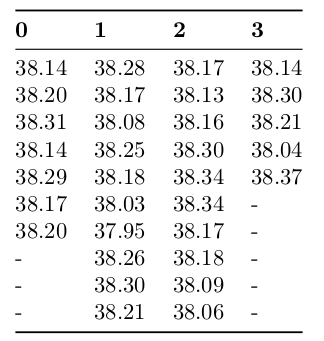
\includegraphics{1.png}
\caption{}
\end{figure}

Answer the question: ``Does pushing the button make the light change
sooner?''. Clearly state the null and alternative hypotheses, the model
used, and all assumptions in the model. Obtain a test statistic (show
all code and R output), and interpret the results of the test.

    \begin{Verbatim}[commandchars=\\\{\}]
{\color{incolor}In [{\color{incolor}1}]:} r \PY{o}{=} \PY{k+kt}{c}\PY{p}{(}\PY{l+m}{7}\PY{p}{,} \PY{l+m}{10}\PY{p}{,} \PY{l+m}{10}\PY{p}{,} \PY{l+m}{5}\PY{p}{)}
        types \PY{o}{=} \PY{k+kt}{c}\PY{p}{(}\PY{l+m}{0}\PY{p}{,} \PY{l+m}{1}\PY{p}{,} \PY{l+m}{2}\PY{p}{,} \PY{l+m}{3}\PY{p}{)}
        button\PYZus{}pushes\PYZus{}type \PY{o}{=} \PY{k+kp}{as.factor}\PY{p}{(}\PY{k+kt}{c}\PY{p}{(}\PY{k+kp}{rep}\PY{p}{(}types\PY{p}{[}\PY{l+m}{1}\PY{p}{]}\PY{p}{,} r\PY{p}{[}\PY{l+m}{1}\PY{p}{]}\PY{p}{)}\PY{p}{,}
                                \PY{k+kp}{rep}\PY{p}{(}types\PY{p}{[}\PY{l+m}{2}\PY{p}{]}\PY{p}{,} r\PY{p}{[}\PY{l+m}{2}\PY{p}{]}\PY{p}{)}\PY{p}{,}
                                \PY{k+kp}{rep}\PY{p}{(}types\PY{p}{[}\PY{l+m}{3}\PY{p}{]}\PY{p}{,} r\PY{p}{[}\PY{l+m}{3}\PY{p}{]}\PY{p}{)}\PY{p}{,}
                                \PY{k+kp}{rep}\PY{p}{(}types\PY{p}{[}\PY{l+m}{4}\PY{p}{]}\PY{p}{,} r\PY{p}{[}\PY{l+m}{4}\PY{p}{]}\PY{p}{)}\PY{p}{)}\PY{p}{)}
        waiting\PYZus{}time \PY{o}{=} \PY{k+kt}{c}\PY{p}{(}\PY{l+m}{38.14}\PY{p}{,} \PY{l+m}{38.20}\PY{p}{,} \PY{l+m}{38.31}\PY{p}{,} \PY{l+m}{38.14}\PY{p}{,} \PY{l+m}{38.29}\PY{p}{,} \PY{l+m}{38.17}\PY{p}{,} \PY{l+m}{38.20}\PY{p}{,} 
                        \PY{l+m}{38.28}\PY{p}{,} \PY{l+m}{38.17}\PY{p}{,} \PY{l+m}{38.08}\PY{p}{,} \PY{l+m}{38.25}\PY{p}{,} \PY{l+m}{38.18}\PY{p}{,} \PY{l+m}{38.03}\PY{p}{,} \PY{l+m}{37.95}\PY{p}{,} \PY{l+m}{38.26}\PY{p}{,} \PY{l+m}{38.30}\PY{p}{,} \PY{l+m}{38.21}\PY{p}{,}
                        \PY{l+m}{38.17}\PY{p}{,} \PY{l+m}{38.13}\PY{p}{,} \PY{l+m}{38.16}\PY{p}{,} \PY{l+m}{38.30}\PY{p}{,} \PY{l+m}{38.34}\PY{p}{,} \PY{l+m}{38.34}\PY{p}{,} \PY{l+m}{38.17}\PY{p}{,} \PY{l+m}{38.18}\PY{p}{,} \PY{l+m}{38.09}\PY{p}{,} \PY{l+m}{38.06}\PY{p}{,}
                        \PY{l+m}{38.14}\PY{p}{,} \PY{l+m}{38.30}\PY{p}{,} \PY{l+m}{38.21}\PY{p}{,} \PY{l+m}{38.04}\PY{p}{,} \PY{l+m}{38.37}\PY{p}{)}
        pedestrian \PY{o}{=} \PY{k+kt}{data.frame}\PY{p}{(}button\PYZus{}pushes\PYZus{}type\PY{p}{,} waiting\PYZus{}time\PY{p}{)}
        pedestrian\PY{p}{[}\PY{k+kp}{sample}\PY{p}{(}\PY{k+kp}{nrow}\PY{p}{(}pedestrian\PY{p}{)}\PY{p}{,} \PY{l+m}{10}\PY{p}{)}\PY{p}{,} \PY{p}{]}
\end{Verbatim}

    \begin{tabular}{r|ll}
  & button\_pushes\_type & waiting\_time\\
\hline
	23 & 2     & 38.34\\
	6 & 0     & 38.17\\
	16 & 1     & 38.30\\
	19 & 2     & 38.13\\
	10 & 1     & 38.08\\
	27 & 2     & 38.06\\
	24 & 2     & 38.17\\
	17 & 1     & 38.21\\
	11 & 1     & 38.25\\
	1 & 0     & 38.14\\
\end{tabular}



\noindent    The first hypothesis tested in the experiment would be that if there is
any difference in the waiting time when pushing different buttons. So if
the waiting time of n times of button pushing turns out to be the same,
that it would indicate that fact that pushing buttons does not actually
shorten the waiting time, thus not making the light changing faster. 
\\\\
So
denote the waiting time as \(\tau\), this is expressed as 

the null
hypothesis:

\[H_0: \tau_0 = \tau_1 = \tau_2 = \tau_3\]

the alternative hypothesis:

\[H_1: \text{at least there's one among the 4 \(\tau_i\) that's different
from the others} \]


\noindent Then we apply the AVOVA model and do pairwise contrasts among each two treatments, calculate the p values adjusted by the tukey method from each contrast.

    \begin{Verbatim}[commandchars=\\\{\}]
{\color{incolor}In [{\color{incolor}5}]:} \PY{k+kn}{library}\PY{p}{(}lsmeans\PY{p}{)}
        aov.pedestrian \PY{o}{=} aov\PY{p}{(}waiting\PYZus{}time\PY{o}{\PYZti{}}button\PYZus{}pushes\PYZus{}type\PY{p}{,} data \PY{o}{=} pedestrian\PY{p}{)}
        lsm.pedestrian\PY{o}{=}lsmeans\PY{p}{(}aov.pedestrian\PY{p}{,} \PY{o}{\PYZti{}} button\PYZus{}pushes\PYZus{}type\PY{p}{)}
        \PY{k+kp}{summary}\PY{p}{(}contrast\PY{p}{(}lsm.pedestrian\PY{p}{,} method\PY{o}{=}\PY{l+s}{\PYZdq{}}\PY{l+s}{pairwise\PYZdq{}}\PY{p}{,} adjust\PY{o}{=}\PY{l+s}{\PYZdq{}}\PY{l+s}{tukey\PYZdq{}}\PY{p}{)}\PY{p}{,}
                        infer\PY{o}{=}\PY{k+kt}{c}\PY{p}{(}\PY{n+nb+bp}{T}\PY{p}{,}\PY{n+nb+bp}{T}\PY{p}{)}\PY{p}{,} level\PY{o}{=}\PY{l+m}{0.95}\PY{p}{,} side\PY{o}{=}\PY{l+s}{\PYZdq{}}\PY{l+s}{two\PYZhy{}sided\PYZdq{}}\PY{p}{)}
\end{Verbatim}

    \begin{tabular}{r|llllllll}
 contrast & estimate & SE & df & lower.CL & upper.CL & t.ratio & p.value\\
\hline
	 0 - 1        &  0.036142857 & 0.05151381   & 28           & -0.1045059   & 0.1767916    &  0.70161489  & 0.8955744   \\
	 0 - 2        &  0.013142857 & 0.05151381   & 28           & -0.1275059   & 0.1537916    &  0.25513269  & 0.9940396   \\
	 0 - 3        & -0.004857143 & 0.06120753   & 28           & -0.1719728   & 0.1622585    & -0.07935532  & 0.9998162   \\
	 1 - 2        & -0.023000000 & 0.04674802   & 28           & -0.1506367   & 0.1046367    & -0.49199943  & 0.9602303   \\
	 1 - 3        & -0.041000000 & 0.05725440   & 28           & -0.1973224   & 0.1153224    & -0.71610217  & 0.8898585   \\
	 2 - 3        & -0.018000000 & 0.05725440   & 28           & -0.1743224   & 0.1383224    & -0.31438632  & 0.9890012   \\
\end{tabular}


    
    \paragraph{Alternatively}\label{alternatively}

    \begin{Verbatim}[commandchars=\\\{\}]
{\color{incolor}In [{\color{incolor}6}]:} TukeyHSD\PY{p}{(}aov.pedestrian\PY{p}{,} \PY{l+s}{\PYZdq{}}\PY{l+s}{button\PYZus{}pushes\PYZus{}type\PYZdq{}}\PY{p}{)}
\end{Verbatim}

    
    \begin{verbatim}
  Tukey multiple comparisons of means
    95% family-wise confidence level

Fit: aov(formula = waiting_time ~ button_pushes_type, data = pedestrian)

$button_pushes_type
            diff        lwr       upr     p adj
1-0 -0.036142857 -0.1767916 0.1045059 0.8955744
2-0 -0.013142857 -0.1537916 0.1275059 0.9940396
3-0  0.004857143 -0.1622585 0.1719728 0.9998162
2-1  0.023000000 -0.1046367 0.1506367 0.9602303
3-1  0.041000000 -0.1153224 0.1973224 0.8898585
3-2  0.018000000 -0.1383224 0.1743224 0.9890012

    \end{verbatim}

    
    \begin{Verbatim}[commandchars=\\\{\}]
{\color{incolor}In [{\color{incolor}7}]:} plot\PY{p}{(}TukeyHSD\PY{p}{(}aov.pedestrian\PY{p}{)}\PY{p}{)}
\end{Verbatim}

    \begin{center}
    \adjustimage{max size={0.5\linewidth}{0.5\paperheight}}{output_7_0.png}
    \end{center}
    { \hspace*{\fill} \\}
    
\noindent    Here we can see that the p values of all the pairwise difference are all
\(\gg 0.05\), thus it does not fall into the rejection region. So with
the significance level of 95\%, we could reach the conclusion that the
waiting time of pushing any buttons, no matter how many pushes of the
button, is not significantly different from each other, indicating 
we have no confidence to state that pushing the button will make the
light change sooner.

    \subsubsection*{Q2}\label{q2}

    \textbf{Hot Dogs} A study was conducted to compare the calories and
sodium in hot dogs made with different types of meat.

    \paragraph{(a)}\label{a}

    Read the data into R and plot calories as a response variable with the
type of meat on the x-axis. Your plot could be either a boxplot or a
plot with one dot for each hot dog.

    \begin{Verbatim}[commandchars=\\\{\}]
{\color{incolor}In [{\color{incolor}2}]:} r \PY{o}{=} \PY{k+kt}{c}\PY{p}{(}\PY{l+m}{20}\PY{p}{,} \PY{l+m}{17}\PY{p}{,} \PY{l+m}{17}\PY{p}{)}
        types \PY{o}{=} \PY{k+kt}{c}\PY{p}{(}\PY{l+s}{\PYZsq{}}\PY{l+s}{Beef\PYZsq{}}\PY{p}{,} \PY{l+s}{\PYZsq{}}\PY{l+s}{Pork\PYZsq{}}\PY{p}{,} \PY{l+s}{\PYZsq{}}\PY{l+s}{Chicken\PYZsq{}}\PY{p}{)}
        protein\PYZus{}type \PY{o}{=} \PY{k+kp}{as.factor}\PY{p}{(}\PY{k+kt}{c}\PY{p}{(}\PY{k+kp}{rep}\PY{p}{(}types\PY{p}{[}\PY{l+m}{1}\PY{p}{]}\PY{p}{,} r\PY{p}{[}\PY{l+m}{1}\PY{p}{]}\PY{p}{)}\PY{p}{,}
                                \PY{k+kp}{rep}\PY{p}{(}types\PY{p}{[}\PY{l+m}{2}\PY{p}{]}\PY{p}{,} r\PY{p}{[}\PY{l+m}{2}\PY{p}{]}\PY{p}{)}\PY{p}{,}
                                \PY{k+kp}{rep}\PY{p}{(}types\PY{p}{[}\PY{l+m}{3}\PY{p}{]}\PY{p}{,} r\PY{p}{[}\PY{l+m}{3}\PY{p}{]}\PY{p}{)}\PY{p}{)}\PY{p}{)}
        calories \PY{o}{=} \PY{k+kt}{c}\PY{p}{(}\PY{l+m}{186}\PY{p}{,} \PY{l+m}{181}\PY{p}{,} \PY{l+m}{176}\PY{p}{,} \PY{l+m}{149}\PY{p}{,} \PY{l+m}{184}\PY{p}{,} \PY{l+m}{190}\PY{p}{,} \PY{l+m}{158}\PY{p}{,} \PY{l+m}{139}\PY{p}{,} \PY{l+m}{175}\PY{p}{,} \PY{l+m}{148}\PY{p}{,} \PY{l+m}{152}\PY{p}{,} \PY{l+m}{111}\PY{p}{,} \PY{l+m}{141}\PY{p}{,} \PY{l+m}{153}\PY{p}{,} \PY{l+m}{190}\PY{p}{,} \PY{l+m}{157}\PY{p}{,} \PY{l+m}{131}\PY{p}{,} \PY{l+m}{149}\PY{p}{,} \PY{l+m}{135}\PY{p}{,} \PY{l+m}{132}\PY{p}{,}
                    \PY{l+m}{173}\PY{p}{,} \PY{l+m}{191}\PY{p}{,} \PY{l+m}{182}\PY{p}{,} \PY{l+m}{190}\PY{p}{,} \PY{l+m}{172}\PY{p}{,} \PY{l+m}{147}\PY{p}{,} \PY{l+m}{146}\PY{p}{,} \PY{l+m}{139}\PY{p}{,} \PY{l+m}{175}\PY{p}{,} \PY{l+m}{136}\PY{p}{,} \PY{l+m}{179}\PY{p}{,} \PY{l+m}{153}\PY{p}{,} \PY{l+m}{107}\PY{p}{,} \PY{l+m}{195}\PY{p}{,} \PY{l+m}{135}\PY{p}{,} \PY{l+m}{140}\PY{p}{,} \PY{l+m}{138}\PY{p}{,}
                    \PY{l+m}{129}\PY{p}{,} \PY{l+m}{132}\PY{p}{,} \PY{l+m}{102}\PY{p}{,} \PY{l+m}{106}\PY{p}{,} \PY{l+m}{94}\PY{p}{,} \PY{l+m}{102}\PY{p}{,} \PY{l+m}{87}\PY{p}{,} \PY{l+m}{99}\PY{p}{,} \PY{l+m}{107}\PY{p}{,} \PY{l+m}{113}\PY{p}{,} \PY{l+m}{135}\PY{p}{,} \PY{l+m}{142}\PY{p}{,} \PY{l+m}{86}\PY{p}{,} \PY{l+m}{143}\PY{p}{,} \PY{l+m}{152}\PY{p}{,} \PY{l+m}{146}\PY{p}{,} \PY{l+m}{144}\PY{p}{)}
        sodium \PY{o}{=} \PY{k+kt}{c}\PY{p}{(}\PY{l+m}{495}\PY{p}{,} \PY{l+m}{477}\PY{p}{,} \PY{l+m}{425}\PY{p}{,} \PY{l+m}{322}\PY{p}{,} \PY{l+m}{482}\PY{p}{,} \PY{l+m}{587}\PY{p}{,} \PY{l+m}{370}\PY{p}{,} \PY{l+m}{322}\PY{p}{,} \PY{l+m}{479}\PY{p}{,} \PY{l+m}{375}\PY{p}{,} \PY{l+m}{330}\PY{p}{,} \PY{l+m}{300}\PY{p}{,} \PY{l+m}{386}\PY{p}{,} \PY{l+m}{401}\PY{p}{,} \PY{l+m}{645}\PY{p}{,} \PY{l+m}{440}\PY{p}{,} \PY{l+m}{317}\PY{p}{,} \PY{l+m}{319}\PY{p}{,} \PY{l+m}{298}\PY{p}{,} \PY{l+m}{253}\PY{p}{,}
                   \PY{l+m}{458}\PY{p}{,} \PY{l+m}{506}\PY{p}{,} \PY{l+m}{473}\PY{p}{,} \PY{l+m}{545}\PY{p}{,} \PY{l+m}{496}\PY{p}{,} \PY{l+m}{360}\PY{p}{,} \PY{l+m}{387}\PY{p}{,} \PY{l+m}{386}\PY{p}{,} \PY{l+m}{507}\PY{p}{,} \PY{l+m}{393}\PY{p}{,} \PY{l+m}{405}\PY{p}{,} \PY{l+m}{372}\PY{p}{,} \PY{l+m}{144}\PY{p}{,} \PY{l+m}{511}\PY{p}{,} \PY{l+m}{405}\PY{p}{,} \PY{l+m}{428}\PY{p}{,} \PY{l+m}{339}\PY{p}{,}
                   \PY{l+m}{430}\PY{p}{,} \PY{l+m}{375}\PY{p}{,} \PY{l+m}{396}\PY{p}{,} \PY{l+m}{383}\PY{p}{,} \PY{l+m}{387}\PY{p}{,} \PY{l+m}{542}\PY{p}{,} \PY{l+m}{359}\PY{p}{,} \PY{l+m}{357}\PY{p}{,} \PY{l+m}{528}\PY{p}{,} \PY{l+m}{513}\PY{p}{,} \PY{l+m}{426}\PY{p}{,} \PY{l+m}{513}\PY{p}{,} \PY{l+m}{358}\PY{p}{,} \PY{l+m}{581}\PY{p}{,} \PY{l+m}{588}\PY{p}{,} \PY{l+m}{522}\PY{p}{,} \PY{l+m}{545}\PY{p}{)}
        hot\PYZus{}dog \PY{o}{=} \PY{k+kt}{data.frame}\PY{p}{(}protein\PYZus{}type\PY{p}{,} calories\PY{p}{,} sodium\PY{p}{)}
        hot\PYZus{}dog\PY{p}{[}\PY{k+kp}{sample}\PY{p}{(}\PY{k+kp}{nrow}\PY{p}{(}hot\PYZus{}dog\PY{p}{)}\PY{p}{,} \PY{l+m}{10}\PY{p}{)}\PY{p}{,} \PY{p}{]}
\end{Verbatim}

    \begin{tabular}{r|lll}
  & protein\_type & calories & sodium\\
\hline
	52 & Chicken & 152     & 588    \\
	43 & Chicken & 102     & 542    \\
	21 & Pork    & 173     & 458    \\
	13 & Beef    & 141     & 386    \\
	50 & Chicken &  86     & 358    \\
	39 & Chicken & 132     & 375    \\
	6 & Beef    & 190     & 587    \\
	5 & Beef    & 184     & 482    \\
	35 & Pork    & 135     & 405    \\
	22 & Pork    & 191     & 506    \\
\end{tabular}


    
    \begin{Verbatim}[commandchars=\\\{\}]
{\color{incolor}In [{\color{incolor}15}]:} \PY{k+kn}{library}\PY{p}{(}ggplot2\PY{p}{)}
         ggplot\PY{p}{(}hot\PYZus{}dog\PY{p}{,} aes\PY{p}{(}x\PY{o}{=}protein\PYZus{}type\PY{p}{,} y\PY{o}{=}calories\PY{p}{,} color\PY{o}{=}protein\PYZus{}type\PY{p}{)}\PY{p}{)} \PY{o}{+}
                     geom\PYZus{}boxplot\PY{p}{(}\PY{p}{)} \PY{o}{+}
                     ylab\PY{p}{(}\PY{l+s}{\PYZsq{}}\PY{l+s}{calories\PYZsq{}}\PY{p}{)} \PY{o}{+}
                     ggtitle\PY{p}{(}\PY{l+s}{\PYZsq{}}\PY{l+s}{Boxplots of calories of different protein types\PYZsq{}}\PY{p}{)} \PY{o}{+}
                     theme\PY{p}{(}plot.title \PY{o}{=} element\PYZus{}text\PY{p}{(}hjust \PY{o}{=} \PY{l+m}{0.5}\PY{p}{)}\PY{p}{)} \PY{o}{+}
                     ylim\PY{p}{(}\PY{k+kp}{min}\PY{p}{(}hot\PYZus{}dog\PY{o}{\PYZdl{}}calories\PY{p}{)}\PY{l+m}{\PYZhy{}0.05}\PY{p}{,} \PY{k+kp}{max}\PY{p}{(}hot\PYZus{}dog\PY{o}{\PYZdl{}}calories\PY{p}{)}\PY{l+m}{+0.05}\PY{p}{)}
\end{Verbatim}

    
    
    \begin{center}
    \adjustimage{max size={0.6\linewidth}{0.6\paperheight}}{output_14_1.png}
    \end{center}
    { \hspace*{\fill} \\}
    
    \paragraph{(b)}\label{b}

    Answer the following question: ``Are there differences in the average
calories of hot dogs made with different kinds of meat?''. To answer
this question, write down a statistical model (clearly state the
response variable, treatment levels, number of replicates, . . . ),
express the above question as a testable null hypothesis, and report the
p-value of the test statistic under the null hypothesis. Your answer
should include all R code used, and the important R output.
\begin{table}[H]
\centering
\title{Calories}\\\
\begin{tabular}{|l|r|r|r|}
	\toprule
	{} &  Beef &  Pork &  Chicken \\
	\midrule
	0  &   186 &   173 &      129 \\
	1  &   181 &   191 &      132 \\
	2  &   176 &   182 &      102 \\
	3  &   149 &   190 &      106 \\
	4  &   184 &   172 &       94 \\
	5  &   190 &   147 &      102 \\
	6  &   158 &   146 &       87 \\
	7  &   139 &   139 &       99 \\
	8  &   175 &   175 &      107 \\
	9  &   148 &   136 &      113 \\
	10 &   152 &   179 &      135 \\
	11 &   111 &   153 &      142 \\
	12 &   141 &   107 &       86 \\
	13 &   153 &   195 &      143 \\
	14 &   190 &   135 &      152 \\
	15 &   157 &   140 &      146 \\
	16 &   131 &   138 &      144 \\
	17 &   149 &      &         \\
	18 &   135 &      &         \\
	19 &   132 &      &         \\
	\bottomrule
\end{tabular}
\end{table}

    Model:

\begin{itemize}
\tightlist
\item
  Treatment levels:

  \begin{itemize}
  \tightlist
  \item
    Beef
  \item
    Pork
  \item
    Chicken
  \end{itemize}
\item
  Response variable:

  \begin{itemize}
  \tightlist
  \item
    Calories
  \end{itemize}
\item
  number of replicates

  \begin{itemize}
  \tightlist
  \item
    Beef: 20
  \item
    Pork: 17
  \item
    Chicken: 17
  \end{itemize}
\end{itemize}

    \begin{Verbatim}[commandchars=\\\{\}]
{\color{incolor}In [{\color{incolor}14}]:} \PY{k+kn}{library}\PY{p}{(}knitr\PY{p}{)}
         \PY{k+kn}{library}\PY{p}{(}lsmeans\PY{p}{)}
         aov.hotdog \PY{o}{=} aov\PY{p}{(}calories\PY{o}{\PYZti{}}protein\PYZus{}type\PY{p}{,} data \PY{o}{=} hot\PYZus{}dog\PY{p}{)}
         kable\PY{p}{(}anova\PY{p}{(}aov.hotdog\PY{p}{)}\PY{p}{,} format\PY{o}{=}\PY{l+s}{\PYZsq{}}\PY{l+s}{markdown\PYZsq{}}\PY{p}{)}
\end{Verbatim}

\newpage

    
    \begin{verbatim}


|             | Df|   Sum Sq|  Mean Sq|  F value|  Pr(>F)|
|:------------|--:|--------:|--------:|--------:|-------:|
|protein_type |  2| 17692.20| 8846.098| 16.07399| 3.9e-06|
|Residuals    | 51| 28067.14|  550.336|       NA|      NA|
    \end{verbatim}

    
    Denote calories as \(c\),

\begin{itemize}
\tightlist
\item
  Null hypothesis:
\end{itemize}

\[H_0: c_{beef} = c_{pork} = c_{chicken}\]

\begin{itemize}
\tightlist
\item
  Alternative hypothesis:
\end{itemize}

\[H_1: \text{among the three protein types, at least the calories of one
is different from the others} \]
\mbox{}
    \begin{Verbatim}[commandchars=\\\{\}]
{\color{incolor}In [{\color{incolor}15}]:} lsm.hotdog\PY{o}{=}lsmeans\PY{p}{(}aov.hotdog\PY{p}{,} \PY{o}{\PYZti{}} protein\PYZus{}type\PY{p}{)}
         \PY{k+kp}{summary}\PY{p}{(}contrast\PY{p}{(}lsm.hotdog\PY{p}{,} method\PY{o}{=}\PY{l+s}{\PYZdq{}}\PY{l+s}{pairwise\PYZdq{}}\PY{p}{,} adjust\PY{o}{=}\PY{l+s}{\PYZdq{}}\PY{l+s}{tukey\PYZdq{}}\PY{p}{)}\PY{p}{,}
                         infer\PY{o}{=}\PY{k+kt}{c}\PY{p}{(}\PY{n+nb+bp}{T}\PY{p}{,}\PY{n+nb+bp}{T}\PY{p}{)}\PY{p}{,} level\PY{o}{=}\PY{l+m}{0.95}\PY{p}{,} side\PY{o}{=}\PY{l+s}{\PYZdq{}}\PY{l+s}{two\PYZhy{}sided\PYZdq{}}\PY{p}{)}
\end{Verbatim}
\mbox{}

    \begin{tabular}{r|llllllll}
 contrast & estimate & SE & df & lower.CL & upper.CL & t.ratio & p.value\\
\hline
	 Beef - Chicken &  38.085294     & 7.738831       & 51             &  19.40391      &  56.76667      &  4.9213237     & 2.767694e-05  \\
	 Beef - Pork    &  -1.855882     & 7.738831       & 51             & -20.53726      &  16.82550      & -0.2398143     & 9.688129e-01  \\
	 Chicken - Pork & -39.941176     & 8.046454       & 51             & -59.36515      & -20.51720      & -4.9638236     & 2.390087e-05  \\
\end{tabular}

\mbox{}
    
    \begin{Verbatim}[commandchars=\\\{\}]
{\color{incolor}In [{\color{incolor}18}]:} beef\PYZus{}chicken\PYZus{}pvalue \PY{o}{=} \PY{l+m}{2.767694e\PYZhy{}05}
         beef\PYZus{}pork\PYZus{}pvalue \PY{o}{=} \PY{l+m}{9.688129e\PYZhy{}01}
         chicken\PYZus{}pork\PYZus{}pvalue \PY{o}{=} \PY{l+m}{2.390087e\PYZhy{}05}
\end{Verbatim}

    \paragraph{(c)}\label{c}

    Are there significant differences in mean calories between Beef and Pork
hot dogs? What about between Beef and Chicken hot dogs? What about
between Pork and Chicken hot dogs?

    \begin{Verbatim}[commandchars=\\\{\}]
{\color{incolor}In [{\color{incolor}19}]:} beef\PYZus{}pork\PYZus{}pvalue\PY{o}{\PYZlt{}}\PY{l+m}{0.05}
         beef\PYZus{}chicken\PYZus{}pvalue\PY{o}{\PYZlt{}}\PY{l+m}{0.05}
         chicken\PYZus{}pork\PYZus{}pvalue\PY{o}{\PYZlt{}}\PY{l+m}{0.05}
\end{Verbatim}

    FALSE

    
    TRUE

    
    TRUE

    
    We can interpret the results of these tests with the following
statements:

\begin{itemize}
\item
  \begin{enumerate}
  \def\labelenumi{\arabic{enumi}.}
  \tightlist
  \item
    The calories of beef is not significantly different from the
    calories of pork;
  \end{enumerate}
\item
  \begin{enumerate}
  \def\labelenumi{\arabic{enumi}.}
  \setcounter{enumi}{1}
  \tightlist
  \item
    The calories of beef is significantly more than the calories of
    chicken;
  \end{enumerate}
\item
  \begin{enumerate}
  \def\labelenumi{\arabic{enumi}.}
  \setcounter{enumi}{2}
  \tightlist
  \item
    The calories of chicken is significantly less than the calories of
    pork;
  \end{enumerate}
\end{itemize}


    % Add a bibliography block to the postdoc
    
    
    
    \end{document}
